% Intended LaTeX compiler: xelatex
\documentclass[10pt, svgnames]{beamer}
\usepackage{graphicx}
\usepackage{longtable}
\usepackage{wrapfig}
\usepackage{rotating}
\usepackage[normalem]{ulem}
\usepackage{amsmath}
\usepackage{amssymb}
\usepackage{capt-of}
\usepackage{hyperref}
\usetheme{focus}
\author{Sappinandana Akamphon}
\date{\today}
\title{Analysis of Torque Loaded Members}
\subtitle{ME 210: Mechanics of Materials}
\usepackage{booktabs}
\usepackage{pgfplots}
\pgfplotsset{compat=1.18}
\institute{Department of Mechanical Engineering, TSE}
\date{}
\usetikzlibrary{patterns,shapes,arrows}
\hypersetup{
 pdfauthor={Sappinandana Akamphon},
 pdftitle={Analysis of Torque Loaded Members},
 pdfkeywords={},
 pdfsubject={},
 pdfcreator={Emacs 30.0.50 (Org mode 9.6)}, 
 pdflang={English}}
\usepackage{biblatex}

\begin{document}

\begin{frame}[label={sec:org6a5a613}]{\{\}}
\maketitle
\end{frame}

\begin{frame}[label={sec:orgf160d7e}]{What is Torsion?}
\begin{itemize}
\item Twisting of a straight bar loaded by torque (torsional moment)

\item Twisting happens about its longitudinal axis
\end{itemize}
\end{frame}

\begin{frame}[label={sec:org6890e5a}]{State of Stress in Torsion}
\begin{center}
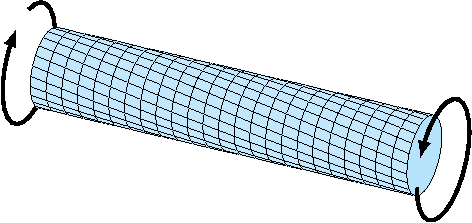
\includegraphics[width=.9\linewidth]{pictures/state-of-torsion-stress.pdf}
\end{center}
\end{frame}

\begin{frame}[label={sec:orgcd23f1f}]{Torsional Deformation in a Circular Bar}
\begin{itemize}
\item When twisted, all cross-section remains circular and subjected to the same torque -- \emph{pure torsion}.

\begin{center}
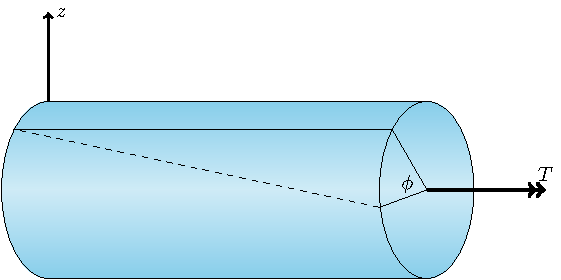
\includegraphics[width=.9\linewidth]{pictures/twisted-bar.pdf}
\end{center}

\item \(\phi\) is called the \emph{angle of twist}, increasing linearly along the length of the bar
\end{itemize}
\end{frame}

\begin{frame}[label={sec:org7e31a74}]{State of Strain in a Twisted Bar}
\begin{itemize}
\item Change in element angle is shear strain

\begin{center}
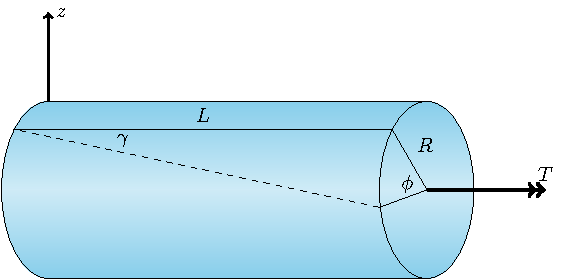
\includegraphics[width=.9\linewidth]{pictures/state-of-strain.pdf}
\end{center}
\end{itemize}

\[\gamma = \frac{Rd\phi}{dx} = R\theta = \frac{R\phi}{L}\]
\end{frame}

\begin{frame}[label={sec:orgc6bcefa}]{Maximum Shear Strain in a Twisted Bar}
\begin{itemize}
\item Maximum shear strain happens at the outer surface
\[\gamma_{\max} = \frac{R \phi}{L}\]

\item What about minimum shear strain? \[\gamma_{\min} = \ldots\]
\end{itemize}
\end{frame}

\begin{frame}[label={sec:org6ec797a}]{State of Stress in a Circular Bar under Torsion}
\begin{columns}
\begin{column}{0.5\columnwidth}
\begin{center}
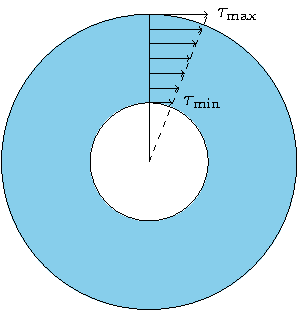
\includegraphics[width=.9\linewidth]{pictures/shear-distribution.pdf}
\end{center}
\end{column}

\begin{column}{0.5\columnwidth}
\begin{itemize}
\item For linear elastic deformation
\end{itemize}

\[\tau = G \gamma\]
\[\tau_{\max} = G\gamma_{\max} = GR \frac{\phi}{L}\]
\[\tau = Gr\frac{\phi}{L} = \tau_{\max} \frac{r}{R}\]
\end{column}
\end{columns}
\end{frame}

\begin{frame}[label={sec:orgcfd9f8c}]{Torsion Formula}
\begin{columns}
\begin{column}{0.5\columnwidth}
\begin{center}
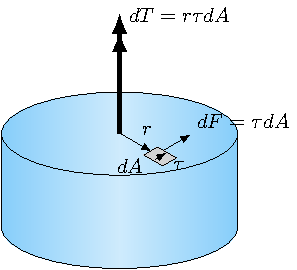
\includegraphics[width=.9\linewidth]{pictures/torsion-formula.pdf}
\end{center}
\end{column}

\begin{column}{0.5\columnwidth}
\begin{gather*}
  dF = \tau dA \\
  dT = r \tau dA = \frac{r^2 \tau_{\max}}{R} dA \\
  \int_0^T dT = \frac{ \tau_{\max} }{R} \int_A r^2 dA = \frac{ \tau_{\max}}{R} J
\end{gather*}

\begin{block}{\small Torsional Shear Stress Formula}
  $$ \tau = \frac{ Tr }{J} $$
\end{block}
\end{column}
\end{columns}
\end{frame}

\begin{frame}[label={sec:orgd3ae352}]{Polar Moment of Inertia: \(J\)}
\begin{itemize}
\item Solid cylindrical shaft
\end{itemize}

\begin{align*}
  I_p &= \int_A r^2 dA \\
      &= \int_0^{2\pi} \int_0^R r^2 r dr d\theta \\
      &= \frac{\pi}{2} R^4
\end{align*}

\begin{itemize}
\item Hollow shaft: how do we do that?
\end{itemize}
\end{frame}

\begin{frame}[label={sec:orgebbbb0f}]{Example: Minimum Shaft Radius}
\begin{center}
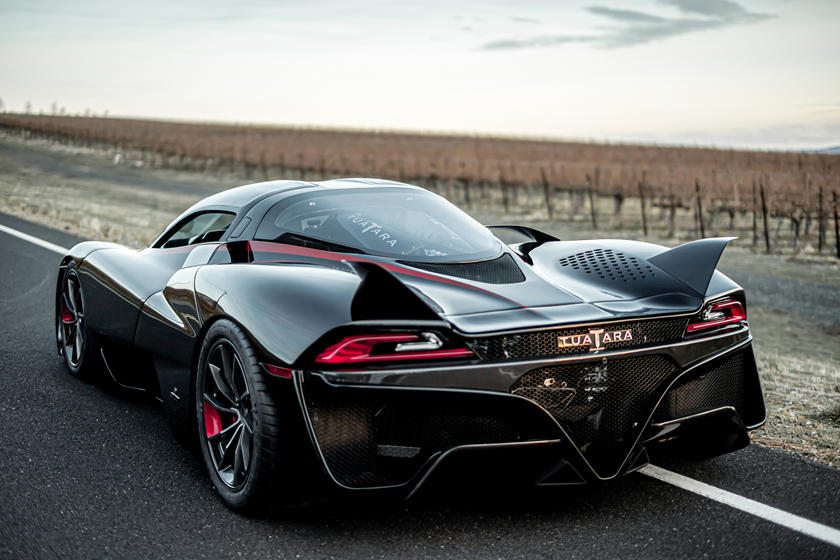
\includegraphics[width=0.7\textwidth]{./pictures/ssc-tuatara.jpg}
\end{center}

\begin{columns}
\begin{column}{0.5\columnwidth}
\begin{align*}
  T_{\max} &= 1735 \text{ N-m} \\
  \tau_{\max} &= 200 \text{ MPa}
\end{align*}
\end{column}

\begin{column}{0.5\columnwidth}
\[r_{\min} = ?\]
\end{column}
\end{columns}
\end{frame}

\begin{frame}[label={sec:orgad6c313}]{Solution: Minimum Required Radius}
\begin{align*}
  \tau &= \frac{Tr}{J} = \frac{2T}{\pi r_{\min}^{3}} \\
  r_{\min} &= \left( \frac{2(1735)}{\pi (200 \times 10^{6})} \right)^{1/3} \\
       &= 0.0177 = 1.77 \text{ cm}
\end{align*}

Isn't that a bit small?
\end{frame}

\begin{frame}[label={sec:org5f1a853}]{Deformation under Torsion: Angle of Twist \(\phi\)}
\begin{itemize}
\item Combine Hooke's law and Torsion formula
\end{itemize}

\[\tau_{\max} = GR\theta = \frac{TR}{J}\]

\begin{gather*}
  \theta = \frac{\phi}{L} = \frac{T}{GJ} \\
  \phi = \frac{TL}{GJ} = \frac{T}{k_T}
\end{gather*}

\begin{itemize}
\item \(k_T\) is called the \emph{torsional stiffness}
\end{itemize}
\end{frame}

\begin{frame}[label={sec:org0ecc5cb}]{Example: Shaft Design}
A gasoline engine has a maximum torque output of 300 N-m. Your boss wants you to design a 2-m long shaft that is going to limit the angle of twist to \(\phi \leqslant\) 0.1 rad. The shaft should be made of medium carbon steel \(G\) = 80 GPa, \(\tau_{\text{allow}}\) = 200 MPa.
\end{frame}

\begin{frame}[label={sec:orgc07e22b}]{Solution: Shaft Design}
Two conditions: \(\tau_{\text{allow}}\) and \(\phi\)

\begin{align*}
  R_{\tau} &= \left( \frac{2T}{\pi \tau_{\text{allow}}} \right)^{1/3} \\
           &= \left( \frac{2(300)}{\pi (200 \times 10^6)} \right)^{1/3} \\
           &= 9.85 \times 10^{-3} \text{ m} = 9.85 \text{ mm} \\
  \phi &= \frac{TL}{GJ} = \frac{2TL}{G \pi R_{\phi}^{4}} \\
  R_{\phi} &= \left( \frac{2(300)(2)}{(80 \times 10^{9})\pi(0.1)} \right)^{1/4} \\
           &= 0.0148 \text{ m} = 1.48 \text{ cm}
\end{align*}

We will need to design based on the bigger requirement, 1.48 cm.
\end{frame}

\begin{frame}[label={sec:orgb5b21df}]{Nonuniform Torsion}
\begin{itemize}
\item \(T\), \(J\), or \(G\) is not constant

\begin{itemize}
\item Segments

\item Continuously varying
\end{itemize}
\end{itemize}
\end{frame}

\begin{frame}[label={sec:org3c93b5e}]{Segments of Constant Values}
\begin{itemize}
\item Determine internal torques and corresponding deformations
\end{itemize}

\begin{center}
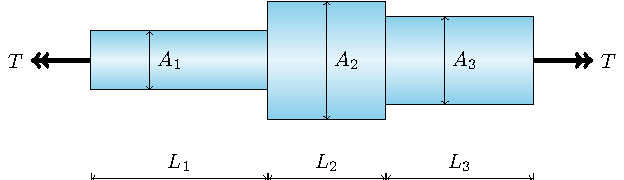
\includegraphics[width=.9\linewidth]{pictures/segments-constant-values.pdf}
\end{center}

\begin{gather*}
  \phi  = {\phi _1} + {\phi _2} + {\phi _3} +  \ldots  \hfill \\
  \phi  = \sum\limits_{i = 1}^n {{\phi _i} = \sum\limits_{i = 1}^n \dfrac{T_iL_i}{G_i J_i} }  \hfill \\
\end{gather*}
\end{frame}

\begin{frame}[label={sec:org9a8fa9e}]{Example: Shaft with Various Segments}
\begin{center}
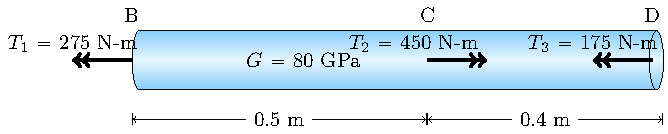
\includegraphics[width=.9\linewidth]{pictures/segments-example.pdf}
\end{center}

\begin{itemize}
\item Find \(\tau_{\max}\) in each segments and \(\phi_{BD}\). Let \(R\) =
1.5 cm.
\end{itemize}
\end{frame}

\begin{frame}[label={sec:orgf88f28c}]{Solution}
Use the method of section to determine torque within segment BC,

\[T_{BC} =  T_1 =  275\text{ Nm}\]

Torque within segment CD,

\[T_{CD} =  T_3 = -175\text{ Nm}\]
\end{frame}

\begin{frame}[label={sec:org4890679}]{Solution}
The maximum shear stress in each segment is at the outer diameter. We have

\begin{gather*}
  \tau _{\max} = \frac{Tr}{J} = \frac{2T}{\pi {r^3}} \hfill \\
  ({\tau_{\max }})_{BC} = \frac{2(275\text{ Nm})}{\pi {(1.5 \times 10^{-2}\text{ m})^3}} = 51.9\text{ MPa} \hfill \\
  ({\tau _{\max }})_{CD} = \frac{2(175\text{ Nm})}{\pi (1.5 \times 10^{-2}\text{ m})^3} = 33\text{ MPa} \hfill
\end{gather*}
\end{frame}

\begin{frame}[label={sec:orgedcbef6}]{Solution}
Angle of twist between B and D is the sum of the angles of twist in BC and CD.

\begin{gather*}
  \phi_{BD} = \phi_{BC} + \phi_{CD} \hfill \\
  J = \frac{\pi r^4}{2} = \frac{\pi (1.5 \times 10^{-2}\text{ m})^4}{2} = 7.95 \times 10^{-8}\text{ m}^4 \hfill \\
  \phi_{BC} = \frac{T_{BC}L_1}{GJ} = \frac{( 275\text{ Nm})(0.5\;{\text{m}})}{(80\text{ GPa})(7.95 \times 10^{-8}\text{ m}^4)} =  0.0216\text{ rad} \hfill \\
  \phi_{CD} = \frac{T_{CD}L_2}{GJ} = \frac{(-175\text{ Nm})(0.4\text{ m})}{(80\text{ GPa})(7.95 \times 10^{-8}\text{ m}^4)} = -0.0110\text{ rad} \hfill \\
  \phi_{BD} =  0.0216 - 0.0110 =  0.0106\text{ rad} \hfill \\
\end{gather*}

Therefore, the bar twisted in the same direction as \(T_2\) by 0.0106
rad.
\end{frame}

\begin{frame}[label={sec:org7cc25f9}]{Continuously Varying Torque / Size / Properties}
\begin{itemize}
\item Back to integration
\end{itemize}

\begin{center}
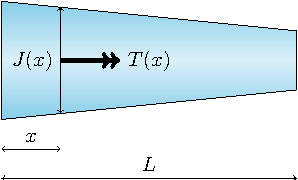
\includegraphics[width=0.6\textwidth]{pictures/cont-vary.pdf}
\end{center}

\begin{align*}
  d\phi &= \frac{T(x) dx}{G(x) J(x)} \\
  \phi  &= \int_0^L \frac{T(x)dx}{G{J(x)}}
\end{align*}
\end{frame}

\begin{frame}[label={sec:org76ec6ba}]{Example: Continuously Varying Shaft}
\begin{center}
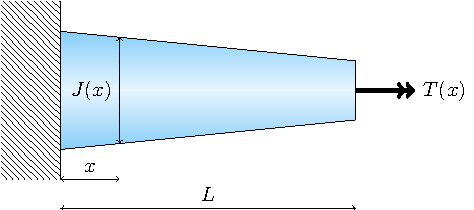
\includegraphics[width=0.9\textwidth]{pictures/cont-vary-example.pdf}
\end{center}

\begin{itemize}
\item What is the total angle of twist \(\phi\)?
\end{itemize}
\end{frame}

\begin{frame}[label={sec:org5443d0e}]{Solution}
\begin{align*}
  \phi &= \int_{0}^{L} \frac{Tdx}{GJ(x)} = \frac{T}{G} \int_{0}^{L} \frac{dx}{J(x)} \\
       &= \frac{T}{G} \int_{0}^{L} \frac{dx}{(\pi/2) \left(\dfrac{r_{2} - r_{1}}{L}x + r_{1}\right)^{4}} \\
       &= \frac{2TL}{3\pi G (r_{2} - r_{1})} \left. \left(\dfrac{r_{2} - r_{1}}{L}x + r_{1}\right)^{-3}  \right|_{0}^{L} \\
       &= \frac{2TL}{3\pi G (r_{2} - r_{1})} \left( -\frac{1}{r_{2}^{3}} + \frac{1}{r_{1}^{3}} \right)
\end{align*}
\end{frame}

\begin{frame}[label={sec:org7d89acd}]{Power Transmission through Shaft}
\begin{itemize}
\item The most important application of shaft is rotational power
transmission
\end{itemize}

\[P = T\omega\]

\begin{itemize}
\item Engine power and speed are typically in \emph{hp} and \emph{rpm}
\end{itemize}

\[1 \text{ hp} = 746 \text{ W}\]
\[1 \text{ rpm} = \frac{2\pi}{60} \text{ rad/s}\]
\end{frame}

\begin{frame}[label={sec:orgd4d21be}]{Example: Shaft Design for an Engine}
\begin{center}
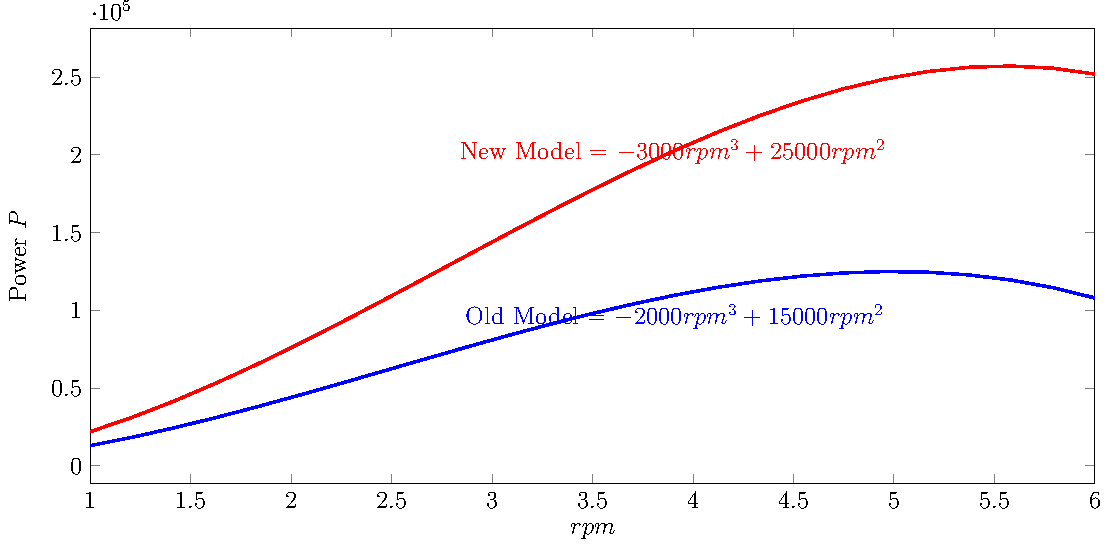
\includegraphics[width=\textwidth]{pictures/shaft-design-example.pdf}
\end{center}

Is it safe to use the old shaft? \(\tau_{allow}\) = 200 MPa.
\end{frame}

\begin{frame}[label={sec:org4ead554}]{Solution}
First order of business is determining maximum torque required.

From \(P = T\omega\)

\begin{align*}
    T_{\text{old}} = -2000 (\frac{2\pi}{60})^{3} \omega^{2} + 15000 (\frac{2\pi}{60})^{2} \omega \\
    T_{\text{new}} = -3000 (\frac{2\pi}{60})^{3} \omega^{2} + 25000 (\frac{2\pi}{60})^{2} \omega
\end{align*}
\end{frame}

\begin{frame}[label={sec:orga955b79}]{Solution Finding max torque is easy now}
\begin{align*}
    \frac{dT_{\text{old}}}{d\omega} = 0 &= -4000 (\frac{2\pi}{60})^{3} \omega + 15000 (\frac{2\pi}{60})^{2}\\
    \omega_{old}^{*} &= \frac{15 \times 60}{4 \times 2\pi} = 35.8 \text{ rad/s} = 342 \text{ rpm} \\
    T_{\text{old,} \max} &= 2945 \text{ N-m} \\
\end{align*}
\end{frame}

\begin{frame}[label={sec:orgb2b97c9}]{Solution}
Max torque for the new engine is

\begin{align*}
    \frac{dT_{\text{new}}}{d\omega} = 0 &= -6000 (\frac{2\pi}{60})^{3} \omega + 25000 (\frac{2\pi}{60})^{2}\\
    \omega_{new}^{*} &= \frac{25 \times 60}{6 \times 2\pi} = 39.8 \text{ rad/s} = 380 \text{ rpm} \\
    T_{\text{new,} \max} &= 5454 \text{ N-m} \\
\end{align*}

Since the new model requires a larger torque, the old shaft will \emph{NOT}
work
\end{frame}

\begin{frame}[label={sec:orgf005eff}]{Solution}
We can now design the new shaft using \(T_{\text{new}}\)
\begin{align*}
    \tau_{max} &= \frac{TR}{J} = \frac{2T}{\pi R^{3}} \\
    R &= \left[ \frac{2(5454)}{\pi ( 200 \times 10^{6} )} \right]^{1/3} \\
               &= 0.026 \text{ m} = 2.6 \text{ cm}
\end{align*}
\end{frame}

\begin{frame}[label={sec:org4a2ddf2}]{Statically Indeterminate Torque-Loaded Members}
\begin{enumerate}
\item Equilibrium equation: torque

\item Compatibility: angle of twist \(\phi\) constraints

\item Hooke's law: relate torque to angle of twist
\end{enumerate}
\end{frame}

\begin{frame}[label={sec:org39ab9f1}]{Example: Compound Shaft}
\begin{center}
\begin{center}
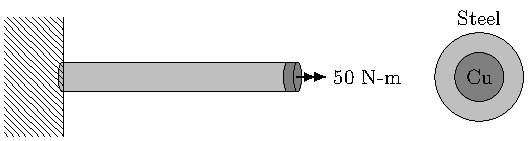
\includegraphics[width=.9\linewidth]{./pictures/compound-shaft.pdf}
\end{center}
\end{center}

\(G_{Cu}\) = 50 GPa \(G_{St}\) = 80 GPa

\begin{enumerate}
\item What is the angle of twist at the end compared to the wall?

\item What is the equivalent shear modulus of the bar?
\end{enumerate}
\end{frame}

\begin{frame}[label={sec:orgc7f6554}]{Solution}
This is a statically indeterminate problem, with the rigid disk
acting as a constraint on the angle of twist of the steel and copper
sections.

1: Equilibrium

\begin{align*}
    T_{\text{cu}} + T_{\text{st}} = 50
\end{align*}
\end{frame}

\begin{frame}[label={sec:orgd6a79c5}]{Solution}
2: Compatibility -- being constrained by the rigid disk, the two materials must rotate by the same amount \(\phi\)

\begin{align*}
  \phi_{\text{cu}} = \phi_{\text{st}} = \phi
\end{align*}

3: Hooke's Law

\begin{gather*}
    \frac{T_{\text{cu}} L}{G_{\text{cu}}J_{\text{cu}}} = \frac{T_{\text{st}}L}{G_{\text{st}} J_{\text{st}}} \\
    T_{\text{cu}} = \frac{50 T_{\text{st}} (\pi/2)(0.05^{4})}{80 (\pi/2)(0.1^{4} - 0.05^{4})} \\
    T_{\text{cu}} = \frac{T_{\text{st}}}{24}
\end{gather*}
\end{frame}

\begin{frame}[label={sec:org1f30022}]{Solution}
Plug back into equilibrium equation,

\begin{align*}
    25 T_{\text{cu}} &= 50 \\
    T_{\text{cu}}  &= 2 \text{ N-m} \\
    T_{\text{st}}  &= 48 \text{ N-m}
\end{align*}

Once we obtained the torques, finding the angle of twist is easy:

\begin{align*}
    \phi &= \frac{T_{\text{cu}} L}{G_{\text{cu}}I_{\text{cu}}} \\
         &= \frac{2(1)}{50 \times 10^{9}(\pi/2)0.05^{4}} \\
         &= 4.08 \times 10^{-6} \text{ rad}
\end{align*}
\end{frame}

\begin{frame}[label={sec:org63b23d2}]{Solution: Equivalent shear modulus}
Similar to equivalent modulus for compound bar:

Given \(T\), find modulus of a single material with same \(J\) and \(L\)
that gives same \(\phi\)

\begin{align*}
    4.08 \times 10^{-6} &= \frac{50(1)}{G_{e}(\pi/2)0.1^{4}} \\
    G_{e} &= 78.1 \times 10^{9} \text{ Pa} = 78.1 \text{ GPa}
\end{align*}
\end{frame}

\begin{frame}[label={sec:org15b6f41}]{Torsion in Thin-walled Tubes}
\begin{columns}
\begin{column}{0.5\columnwidth}
\begin{center}
\begin{center}
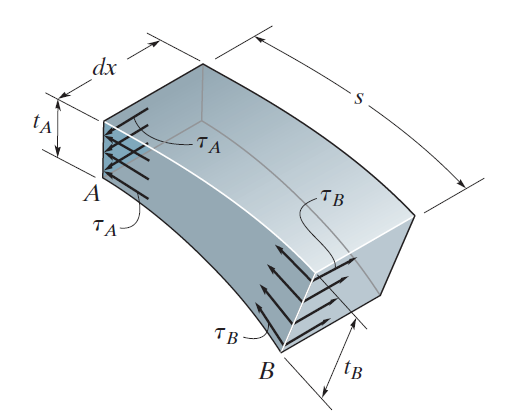
\includegraphics[width=.9\linewidth]{./pictures/thin-walled-tube.png}
\end{center}
\end{center}
\end{column}

\begin{column}{0.5\columnwidth}
\begin{itemize}
\item Equilibrium
\end{itemize}

\[\tau_A t_A dx = \tau_B t_B dx\] \[\tau_A t_A = \tau_B t_B = q\]

\begin{itemize}
\item \(q\) is called \emph{shear flow} and is constant over the cross section

\item \(\tau\) is maximum at the thinnest part
\end{itemize}
\end{column}
\end{columns}
\end{frame}

\begin{frame}[label={sec:org9d59bc4}]{Torsion Formula for Thin-walled Tubes}
\begin{columns}
\begin{column}{0.6\columnwidth}
\begin{center}
\begin{center}
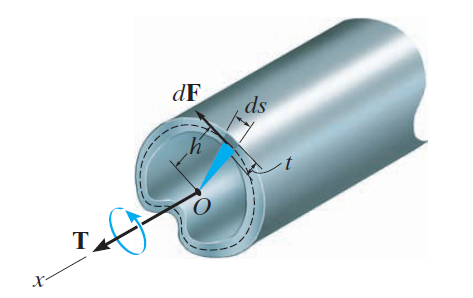
\includegraphics[width=.9\linewidth]{./pictures/thin-walled-torsion-formula.png}
\end{center}
\end{center}
\end{column}

\begin{column}{0.4\columnwidth}
\[dT = rdF = rqds\] \[T = q \oint rds\] \[T = 2 A_m q\]
\[q = \tau t = \frac{T}{2A_m}\]

\[\tau = \frac{T}{2A_m t}\]
\end{column}
\end{columns}
\end{frame}

\begin{frame}[label={sec:org157de5b}]{Angle of Twist in Thin-walled Tube}
\begin{itemize}
\item Derived using energy method
\end{itemize}

\[\phi = \frac{TL}{4A_m^2 G} \oint \frac{ds}{t}\]

\begin{itemize}
\item Intimidating, but actually quite simple

\item For tubes with segments of constant thickness
\end{itemize}

\[\phi = \frac{TL}{4A_m^2 G} \left[ \frac{s_1}{t_1} + \frac{s_2}{t_2} + \ldots \right]\]
\end{frame}

\begin{frame}[label={sec:org3485d22}]{Example: Shear Stress and Angle of Twist in Box Steel}
\begin{center}
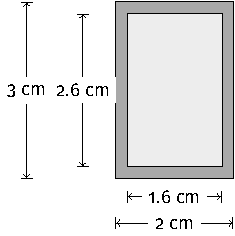
\includegraphics[height=0.5\textheight]{pictures/thin-walled-example.pdf}
\end{center}

\begin{itemize}
\item If the box steel is 2 m long with 20 N-m torque applied, determine
\(\tau_{\max}\) and \(\phi\). Steel has \(G\) = 80 GPa
\end{itemize}
\end{frame}

\begin{frame}[label={sec:org554a56b}]{Solution}
Since the hollow section thickness is constant, \(\tau\) is constant

\begin{align*}
    \tau &= \frac{T}{2 A_{m} t} = \frac{20}{2 (0.018 \times 0.028) (0.002)} \\
         &= 9.92 \text{ MPa} \\
    \phi &= \frac{TL}{4A_{m}^{2}G} \oint \frac{ds}{t} = \frac{20(2)}{4(0.018 \times 0.028)^{2}(80 \times 10^{9})} \left[ \frac{2(0.018+0.028)}{0.002} \right] \\
         &= 2.26 \times 10^{-2} \text{ rad}
\end{align*}
\end{frame}
\end{document}